\subsection{Panorama bibliométrico exploratorio}
\label{sec:res-bibliometria}
% PRISMA ítem 17 (características de los estudios; análisis exploratorio, no preespecificado)

Este panorama bibliométrico es un análisis exploratorio y descriptivo (enmienda A6) que no modifica ninguna conclusión pre-especificada. OpenAlex resolvió \nResueltosOA{} de los \nEstudios{} estudios en la consulta del \fechaOpenalex{}; los \nNoResueltosOA{} restantes no cuentan con datos bibliométricos.
% fuente: bibliometria_resultados.json

% Generado por analysis/src/tablas/figuras_tex.py — no editar a mano.
\begin{figure*}[!tbp]
\centering
\begin{minipage}[b]{0.56\textwidth}\centering
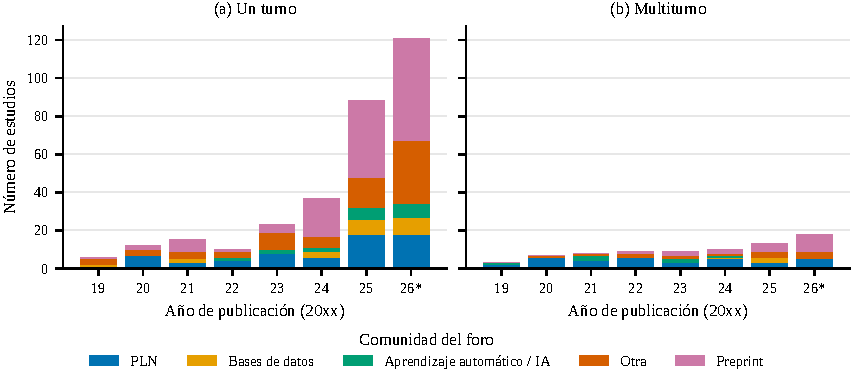
\includegraphics[width=\linewidth]{bib_comunidad}\\(a)\\[3pt]
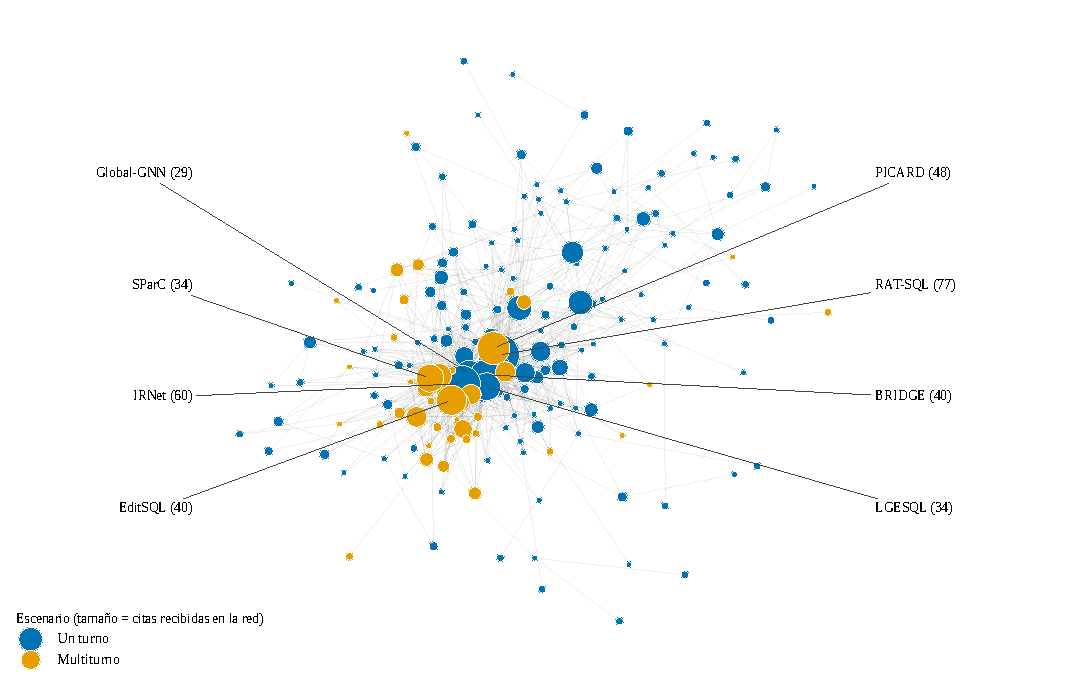
\includegraphics[width=\linewidth]{bib_red_citas}\\(b)
\end{minipage}\hfill
\begin{minipage}[b]{0.42\textwidth}\centering
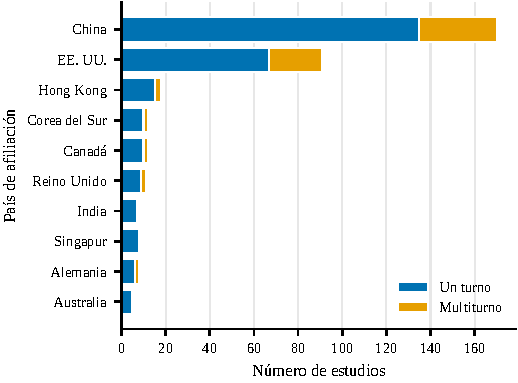
\includegraphics[width=0.82\linewidth]{bib_paises}\\(c)\\[3pt]
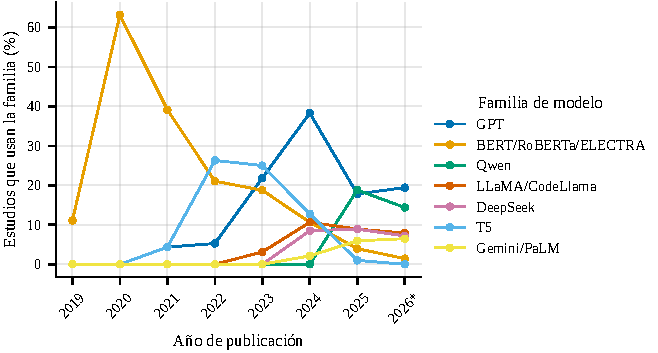
\includegraphics[width=\linewidth]{bib_modelos}\\(d)
\end{minipage}
\caption{Panorama bibliométrico exploratorio (enmienda A6). (a) Comunidad de investigación del foro de publicación, por año: (a) estudios de un turno; (b) estudios multiturno. *2026: año parcial. (b) Red de citas entre los estudios incluidos con al menos un vínculo (184 de 389 estudios; 841 citas; fuente: OpenAlex, 2026-10-13). Etiquetas: los ocho estudios más citados dentro de la red, con su número de citas. (c) Los diez países con más estudios incluidos, por escenario. Un estudio se cuenta en cada país con al menos un autor afiliado (fuente: OpenAlex, 2026-10-13). (d) Familias de modelos base por año (porcentaje de los estudios del año que mencionan la familia; un estudio puede usar varias). En el Nivel 1 solo se registraron los modelos citados en las páginas 1–2, por lo que el uso real está subestimado. *2026: año parcial.}
\label{fig:bib_panorama}
\end{figure*}


El panel~(a) de la \cref{fig:bib_panorama} clasifica el foro de publicación en cinco comunidades. Entre los estudios multiturno, \nComunidadPlnMT{} se publicaron en foros de procesamiento del lenguaje natural, \nComunidadBasesDatosMT{} en foros de bases de datos, \nComunidadAprendizajeMT{} en foros de aprendizaje automático o inteligencia artificial y \nComunidadOtraMT{} en otros foros, y \nComunidadPreprintMT{} son \en{preprints}. Entre los estudios de un turno, las cifras son \nComunidadPlnUT{}, \nComunidadBasesDatosUT{}, \nComunidadAprendizajeUT{}, \nComunidadOtraUT{} y \nComunidadPreprintUT{}, respectivamente.
% fuente: bib_comunidad.csv, PI0.md

La red de citas entre los estudios incluidos (panel~(b)) reúne \nCitasRed{} citas entre \nConVinculo{} estudios con al menos un vínculo, mientras que \nAislados{} estudios quedan aislados. Por dirección, hay \nCitasUTUT{} citas de un turno a un turno, \nCitasUTMT{} de un turno a multiturno, \nCitasMTMT{} de multiturno a multiturno y \nCitasMTUT{} de multiturno a un turno. La mediana de citas por año desde la publicación es de \citasMedMT{} en los estudios multiturno y de \citasMedUT{} en los de un turno. Por tipo de afiliación, \nAfilAcademia{} estudios son solo de academia, \nAfilMixta{} combinan academia e industria, \nAfilIndustria{} son solo de industria y \nAfilSinDatos{} carecen de datos.
% fuente: bibliometria_resultados.json, PI0.md, leyendas.json

Respecto de los países (panel~(c)), China registra 170 estudios (35 multiturno y 135 de un turno) y Estados Unidos 91 (24 y 67); siguen Hong Kong con 18, Corea del Sur con 12 y Canadá con 12. En cuanto a las familias de modelos base (panel~(d)), BERT, RoBERTa y ELECTRA y T5 son las más mencionadas hasta 2022; GPT lo es en 2024 y en 2026, y Qwen en 2025. Claude y Qwen aparecen desde 2025, y DeepSeek desde 2024. En el Nivel 1 solo se registraron los modelos citados en las páginas 1 y 2, de modo que el uso real de cada familia está subestimado, y las cifras por país y por comunidad dependen de la cobertura de OpenAlex y de la clasificación de los foros.
% fuente: bib_paises.csv, bib_modelos_anio.csv, PI0.md

Los análisis de productividad y red de coautoría, y de frecuencia de términos en títulos y resúmenes, se publican en el repositorio del proyecto.
